%generare il pdf con il comando: pdflatex main.tex
\documentclass[a4paper, oneside, openany, dvipsnames, table]{article}
\usepackage{../template/SWEightStyle}
\usepackage{tabularx}
\usepackage{ltablex}
\usepackage{hyperref}
\usepackage{verbatim}
\newcommand{\Titolo}{Manuale Utente}

\newcommand{\Gruppo}{SWEight}

\newcommand{\Approvatore}{Damien Ciagola}
\newcommand{\Redattori}{Alberto Bacco \newline Sebastiano Caccaro \newline Gheorghe Isachi \newline Gionata Legrottaglie}
\newcommand{\Verificatori}{Francesco Corti \newline Francesco Magarotto}

\newcommand{\pathimg}{../template/img/logoSWEight.png}

\newcommand{\Versionedoc}{1.0.0}

\newcommand{\Distribuzione}{\proponente \newline Prof. Vardanega Tullio \newline Prof. Cardin Riccardo \newline Gruppo SWEight}

\newcommand{\Uso}{Esterno}

\newcommand{\NomeProgetto}{Colletta}

\newcommand{\Mail}{SWEightGroup@gmail.com}

\newcommand{\DescrizioneDoc}{Questo documento si occupa di fornire le modalità di utilizzo del software Colletta commissionato}


\begin{document}
\copertina{} 
\definecolor{greySWEight}{RGB}{255, 71, 87}
\definecolor{greyROwSWEight}{RGB}{234, 234, 234}

\section*{Registro delle modifiche}
{
	\rowcolors{2}{greyROwSWEight}{white}
	\renewcommand{\arraystretch}{1.5}
	\centering
	\begin{longtable}{ c c C{4cm}  c  c }
		
		\rowcolor{greySWEight}
		\textcolor{white}{\textbf{Versione}} & \textcolor{white}{\textbf{Data}} & \textcolor{white}{\textbf{Descrizione}} & \textcolor{white}{\textbf{Nominativo}} & \textcolor{white}{\textbf{Ruolo}}\\
		1.2.2 & 2019-02-25 & Ampliamento sezione 5.4 e 3.2.5.2 & Alberto Bacco & \reda{} \\
		
		1.2.1 & 2019-02-23 & Aggiunta sezione 3.2.5.8 Checkstyle & Sebastiano Caccaro & \reda{} \\		
		
		1.2.0 & 2019-02-20 & Aggiunta scelte tecnologiche 3.2.4.2, da 3.4.5.4 a 3.4.5.7, 4.3.1.4, 4.3.2.2, 4.4.6 e figlie & Sebastiano Caccaro & \reda{} \\	
		
		1.1.5 & 2019-02-20 & Modifica sezione 2 & Alberto Bacco & \reda{} \\
		
		1.1.4 & 2019-02-18 & Correzione errori grammatica, spostate sottosezioni di asana da 4.3 a 5.2, & Alberto Bacco & \reda{} \\
		
		1.1.3 & 2019-02-14 & Riorganizzazione e correzione errori sezione 5 & Enrico Muraro & \reda{} \\
		
		1.1.2 & 2019-02-03 & Modifica sottosezione 4.1.10, 4.3.1.4, 4.3.1.5, 4.3.1.6 & Alberto Bacco& \reda{} \\	
		
		1.1.1 & 2019-01-31 & Modifica struttura e contenuti sezione 3  & Damien Ciagola & \reda{} \\	
		
		1.1.0 & 2019-01-27 & Sezione Qualità 4.2 & Sebastiano Caccaro & \reda{} \\	
		
		1.0.1 & 2019-01-25 & Parziale ristrutturazione della struttura del documento & Sebastiano Caccaro & \reda{} \\		
		
		1.0.0 & 2019-01-11 & Approvazione per il rilascio & Sebastiano Caccaro & \Res{} \\
		
		0.9.0 & 2019-01-9 & Verifica finale & Francesco Corti & \ver{} \\
		
		0.9.0 & 2019-01-8 & Aggiunta lista di controllo & Gionata Legrottaglie & \reda{} \\
		
		0.8.0 & 2018-12-23 & Correzioni errori ortografici & Gionata Legrottaglie & \reda{} \\
		
		0.7.0 & 2018-12-20 & Verifica documento & Francesco Corti & \ver{}\\
		
		0.6.0 & 2018-12-18 & Aggiunta sottosezione 5.2.2.2, 5.2.2.3, 5.2.2.4 & Francesco Magarotto & \reda{} \\
		
		0.5.2 & 2018-12-16 & Modifica sezione 4.1.5.3 & Alberto Bacco & \reda{} \\
		
		0.5.2 & 2018-12-16 & Modifica sezione 4.1.5.3 & Alberto Bacco & \reda{} \\
		
		0.5.2 & 2018-12-16 & Aggiunte sottosezioni  & Alberto Bacco & \reda{} \\
		
		0.5.1 & 2018-12-15 & Aggiunte sottosezioni 5.3, 5.4, 5.5, 5.6, 5.7, 5.8 & Alberto Bacco & \reda{} \\
		
		0.5.0 & 2018-12-15 & Aggiunta sezione 5 e sottosezioni 5.1, 5.2 & Gionata Legrottaglie & \reda{} \\
		
		0.4.1 & 2018-12-11 & Aggiunta sezione 4.1.7.3.1 & Francesco Magarotto & \reda{} \\ 
		
		0.4.0 & 2018-12-10 & Aggiunte sottosezioni 4.1.5, 4.1.6, 4.1.7, 4.1.8 & Gionata Legrottaglie & \reda{} \\ 
		0.4.0 & 2018-12-09 & Aggiunta sezione 4 e sottosezioni 4.1.1, 4.1.2, 4.1.3, 4.1.4 & Gionata Legrottaglie & \reda{} \\ 
		
		0.3.1 & 2018-12-07 & Aggiunta sottosezione 3.2 & Gionata Legrottaglie & \reda{} \\ 
		
		0.3.0 & 2018-12-06 & Aggiunta sezione 3 e sottosezione 3.1 & Gionata Legrottaglie & \reda{} \\ 
		
		0.2.0 & 2018-12-05 & Aggiunti i riferimenti & Gionata Legrottaglie & \reda{} \\ 
		
		0.1.0 & 2018-11-30 & Aggiunta introduzione & Gionata Legrottaglie & \reda{} \\
		
		0.0.1 & 2018-11-28 & Creazione scheletro del documento & Gionata Legrottaglie & \reda{}\\
		
	\end{longtable}

}
\newpage
\tableofcontents
\newpage
\listoffigures
\newpage
\listoftables
\newpage

\section{Introduzione}
\subsection{Document goal}
The purpose of this document is to provide all the necessary information to extend, correct and improve Colletta.
There will be additional information regarding setting up the development environment to work in an environment that is as consistent as possible with that used
by the other members of group SWEight, but can be ignored if you only want to use part of the product.
This guide was written taking into account the Microsoft Windows and Linux operating systems. If other systems are used, compatibility issues may arise, even if it's unlikely. In this case refer to the git page. This document will grow as the product will be fully
developed.

\subsection{Product goal}
The purpose of the product is the creation of a collaborative data collection platform where users can prepare and/or perform small grammar exercises. 
The front-end of the system consists of a web application developed with React and Redux, while the back-end is a Spring Boot application written in Java, which will handle HTTP Requests sent from the front-end. 

\subsection{References}


\subsubsection{Installation references}

\begin{itemize}
\item \textbf{Git}: \url{https://git-scm.com/}
\item \textbf{Node.js}: \url{https://nodejs.org/en/}
\item \textbf{NPM}: \url{https://www.npmjs.com/}
\item \textbf{Oracle JDK}: \url{https://www.oracle.com/technetwork/java/javase/downloads/index.html}
\item \textbf{OpenJDK}: \url{https://openjdk.java.net/}
\item \textbf{Maven}: \url{https://maven.apache.org/}
\item \textbf{Lombok}: \url{https://projectlombok.org/}
\item \textbf{VSCode}: \url{https://code.visualstudio.com/} 

\end{itemize}

\subsubsection{Legal references}
\begin{itemize}
\item \textbf{MIT License}: \url{https://opensource.org/licenses/MIT}
\end{itemize}

%\subsubsection{Informative references}

\newpage
\section{Installazione ed esecuzione}
Il codice relativo alla Product Baseline lo si può trovare al seguente link:
\begin{center}
\href{https://github.com/SWEightgroup/Development}{Colletta}. 
\end{center}

\subsection{Maven project}
Una volta fatto il clone della repository o dopo aver scaricato lo zip, posizionarsi nella directory "Mockup-V2/Backend" della repo e utilizzare i seguenti comandi:

\begin{center}
\textsf{mvn clean install}
\end{center}

\begin{center}
\textsf{mvn exec:java}
\end{center}

\subsection{Node.js}
Per lo sviluppo del front-end ci si avvale dell’ultima versione Long Term Support (LTS) di Node.js, che, al momento della stesura di questo documento, è la 10.15.1 LTS. Node.js è reperibile al
seguente link:

\begin{center}
\href{https://nodejs.org/it/}{Node.js}. 
\end{center}

Il file package.json contiene tutte le configurazioni e dipendenze del progetto. Per installare tutti i moduli
necessari è necessario eseguire il seguente comando nella cartella contenente il file package.json:
\begin{center}
\textsf{npm install}
\end{center}
Per eseguire il progetto è necessario usare il comando:
\begin{center}
\textsf{npm start}
\end{center}

\newpage
\section{Architettura del prodotto}
\subsection{MongoDB Database}
\begin{figure}[H]
\centering
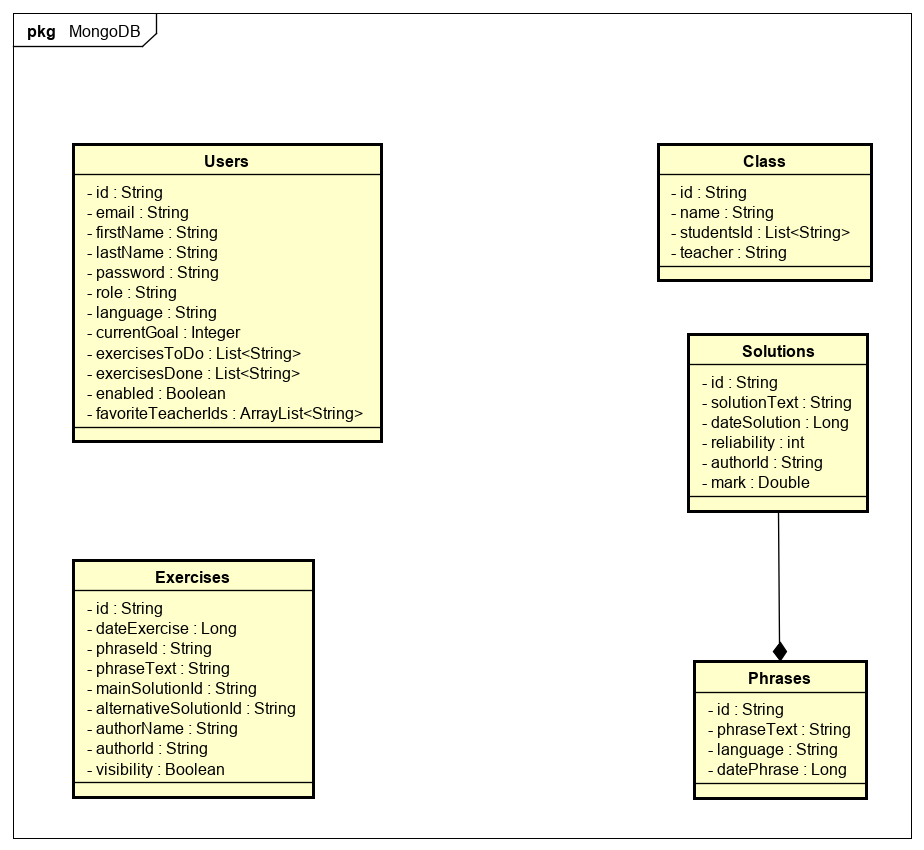
\includegraphics[width=17cm, keepaspectratio]{img/mongodb.png} 
\caption{Exercise insert}
\end{figure}
\subsection{Design pattern utilizzati}
\subsubsection{Backend}
\paragraph{Adapter}
L'utilizzo della libreria di Freeling, per il pos-tagging, ha richiesto la creazione di un Adapter nella variante Object Adapter per poter adattare le funzionalità strettamente necessarie.
\begin{figure}[H]
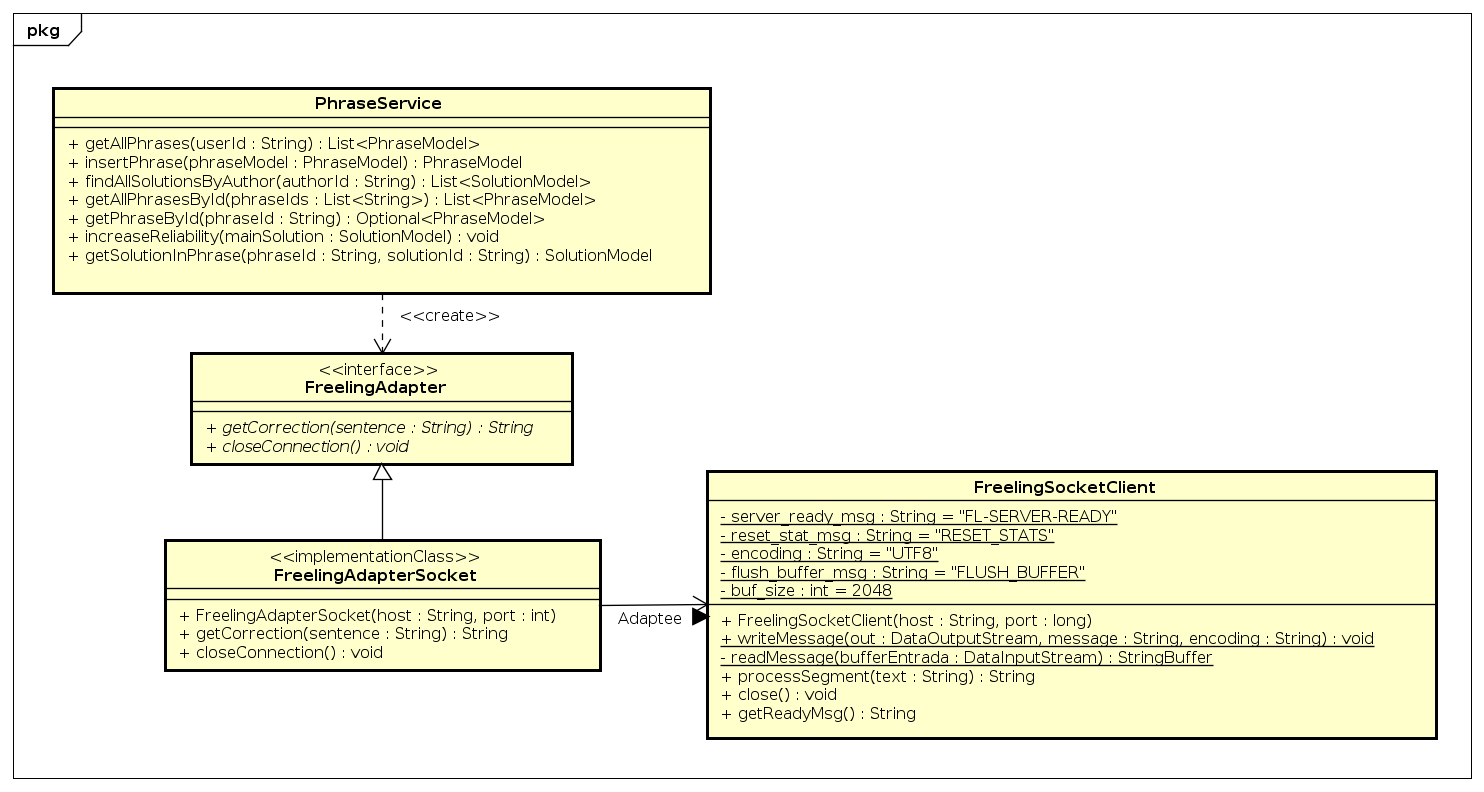
\includegraphics[width=17cm]{img/Adapter.png} 
\caption{Diagramma delle classi Adapter}
\end{figure}
La classe FreelingSocketClient viene fornita dai creatori della libreria e si occupa di realizzare la connessione con il server Freeling scritto in C++.
\paragraph{Controller - Service - Repository - Model}
L'architettura realizzata all'interno di Spring Web consta nella presenza di:
\begin{itemize}
\item \textbf{Controller}: un a cui è delegato il compito di gestire le richieste provenienti dalla parte frontend e alla cattura delle eccezioni;
\item \textbf{Service}: realizzano la business-logic;
\item \textbf{Repository}: realizzano il layer di persistenza gestendo la base di dati;
\item \textbf{Model}: rappresentano oggetti  Plain Old Java Object, un'istanza di un model rappresenta un documento di una collezione.
\end{itemize}
\begin{figure}[H]
\centering
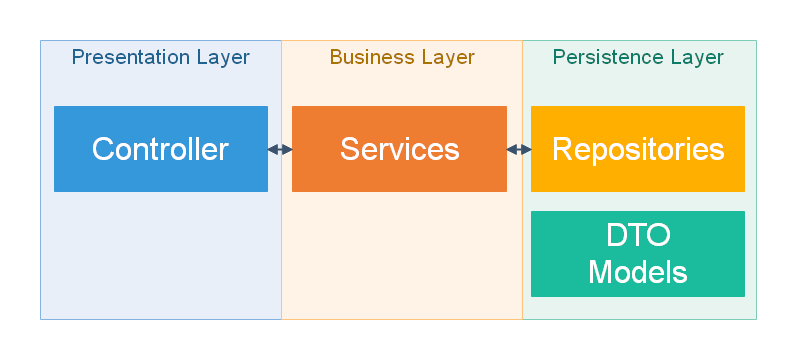
\includegraphics[width=14cm]{img/springArch.png}
\caption{Scherma generale architettura in Spring}
\end{figure}

\subsubsection{Frontend}
\paragraph{Flux}\mbox{}\\

\begin{figure}[H]
    \centering
	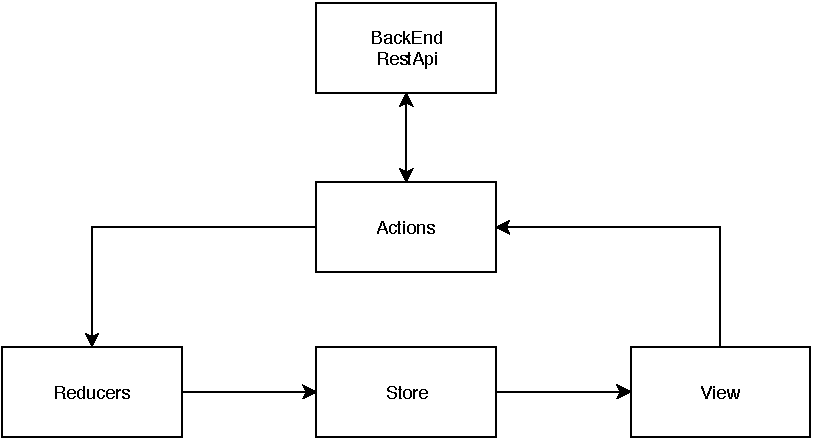
\includegraphics[width=0.7\linewidth]{img/Flux.pdf}
	\caption{Schema del design pattern Flux}
\end{figure}

Per la frontend viene utilizzato React con design pattern Redux, un'evoluzione del design pattern Flux.
In Redux, tutti i dati scorrono in modo unidirezionale attraverso i seguenti componenti:
\begin{itemize}
    \item \textbf{Store: }oggetto immutabile che contiene l'intero stato dell'applicazione in maniera centralizzata;
    \item \textbf{Reducers: }sono funzioni pure. Ogni volta che i Reducer ricevono una nuova azione, 
    processano l'azione ricevuta e, in caso sia necessario apportare delle modifiche allo stato, restituiscono un nuovo oggetto 
    \item \textbf{Action creators: }funzioni che facilitano la gestione del dispatch (creazione di azioni da mandare ai reducers); 
    \item \textbf{View: }componenti grafiche, il loro contenuto dipende dallo store. Sono implementate attraverso un \textit{Observer Pattern} sullo store stesso.
    Ad ogni cambiamento di stato prodotto da un reducers vengono renderizzate le componenti collegate ad esso.
\end{itemize} 


\subsection{Diagrammi dei package}
\subsubsection{Data Transfer Object}
Le classi Helper rappresentano Data Transfer Object (DTO), vengono utilizzate dalla classe \texttt{Controller.java} per fornire un oggetto per il trasferimento dati dalla frontend senza ricorrere a JSON troppo complessi.

\subsubsection{Builder}
I model sono dotati ognuno di un builder, tale classe interna non è codificata ma realizzata tramite un plugin denominato lambok. A seguire viene mostrato un esempio di un builder creato automaticamente.
\begin{figure}[H]
\centering
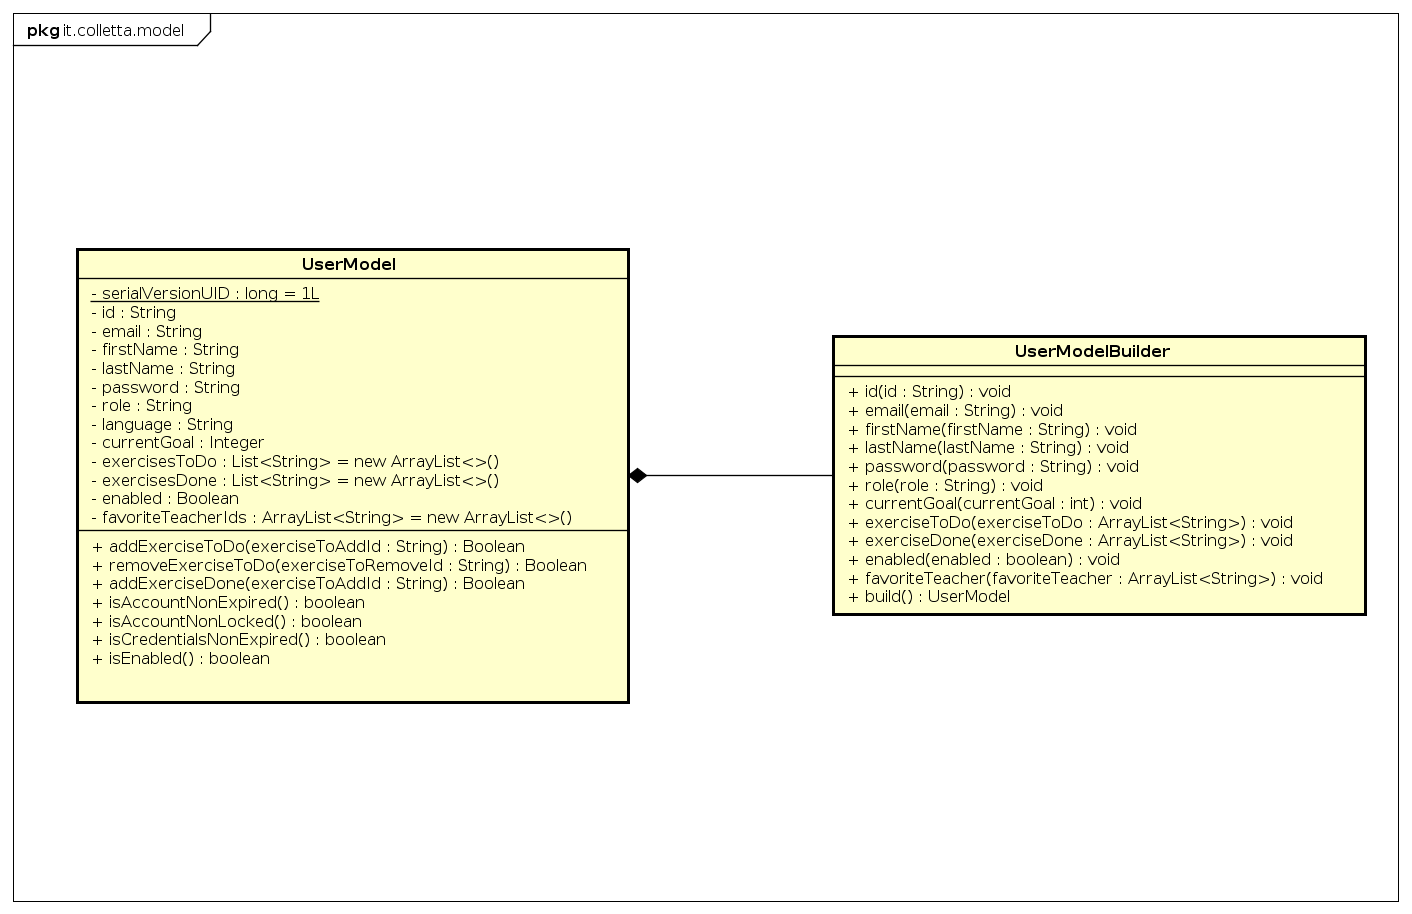
\includegraphics[width=15cm]{img/builder.png}
\caption{Esempio di builder presente nella classe UserModel}
\end{figure}

\subsection{Model}
Viene di seguito riportato il diagramma delle classi del package model.
\begin{figure}[H]
\centering
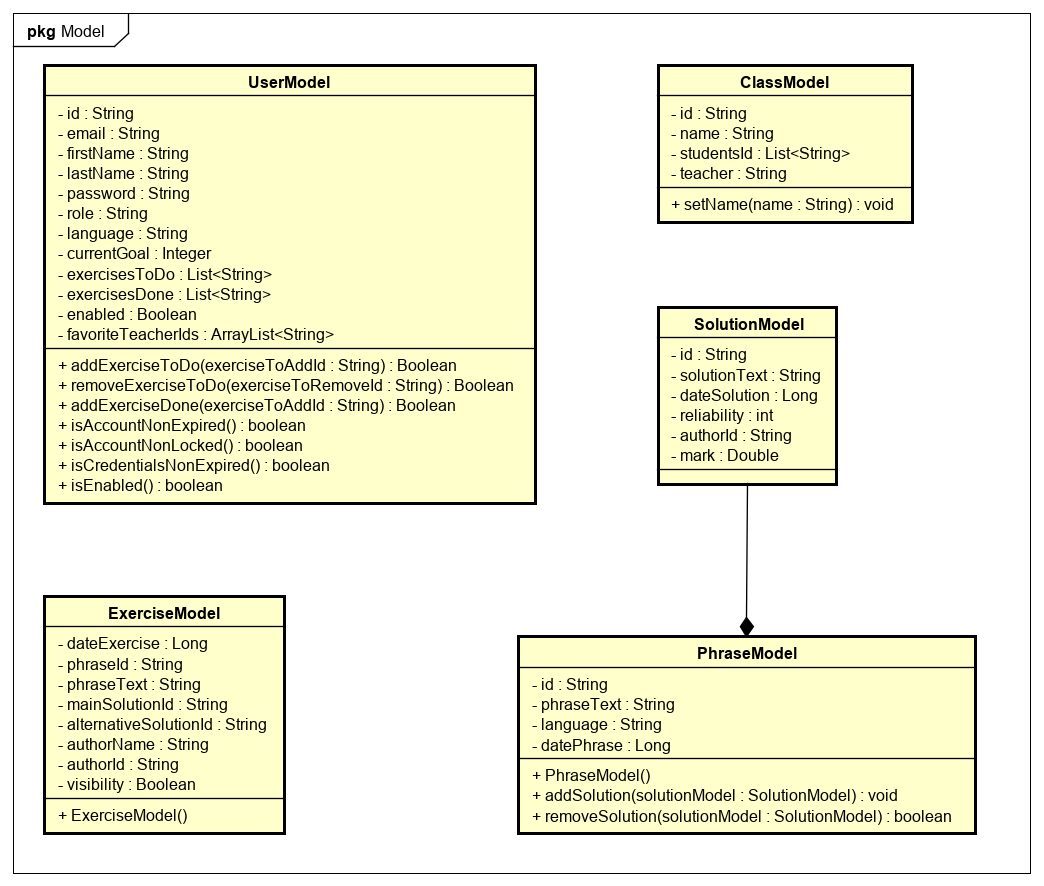
\includegraphics[width=17cm, keepaspectratio]{img/model.png} 
\caption{Model}
\end{figure}
\newpage

\subsection{Controller e service}
Viene di seguito riportato il diagramma delle classi di package controller e service.
\begin{figure}[H]
\centering
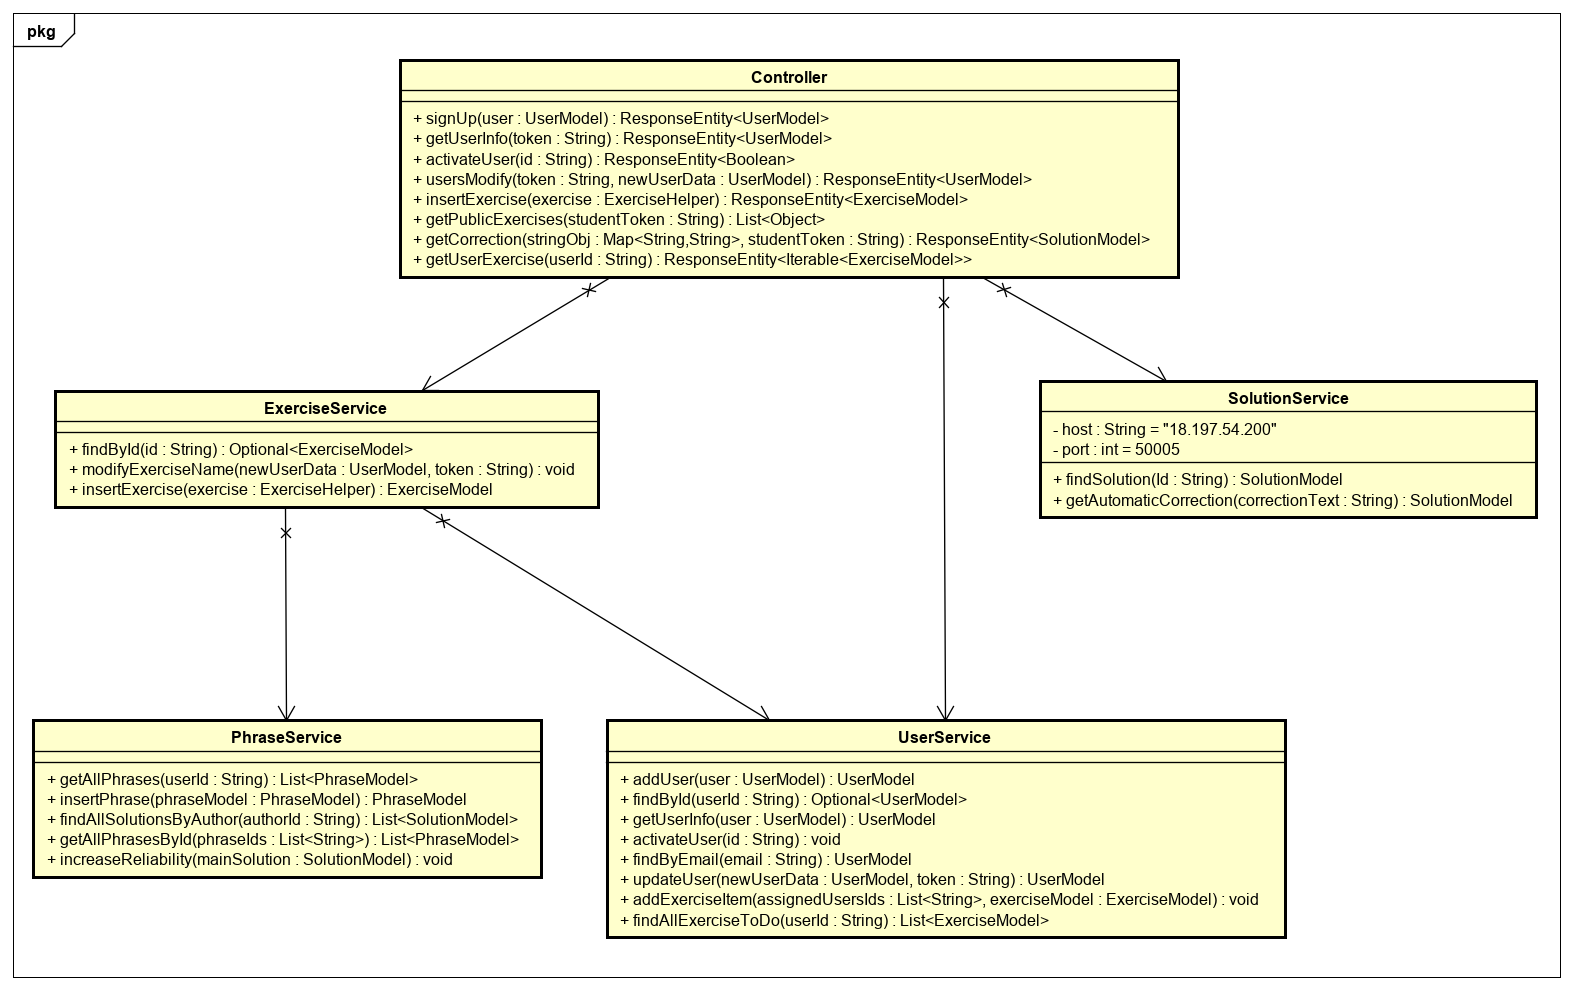
\includegraphics[width=17cm, keepaspectratio]{img/Controller-service.png} 
\caption{Controller e Service}
\end{figure}
\newpage
\subsection{Service e repository}
Viene di seguito riportato il diagramma delle classi di package service e repository.
\begin{figure}[H]
\centering
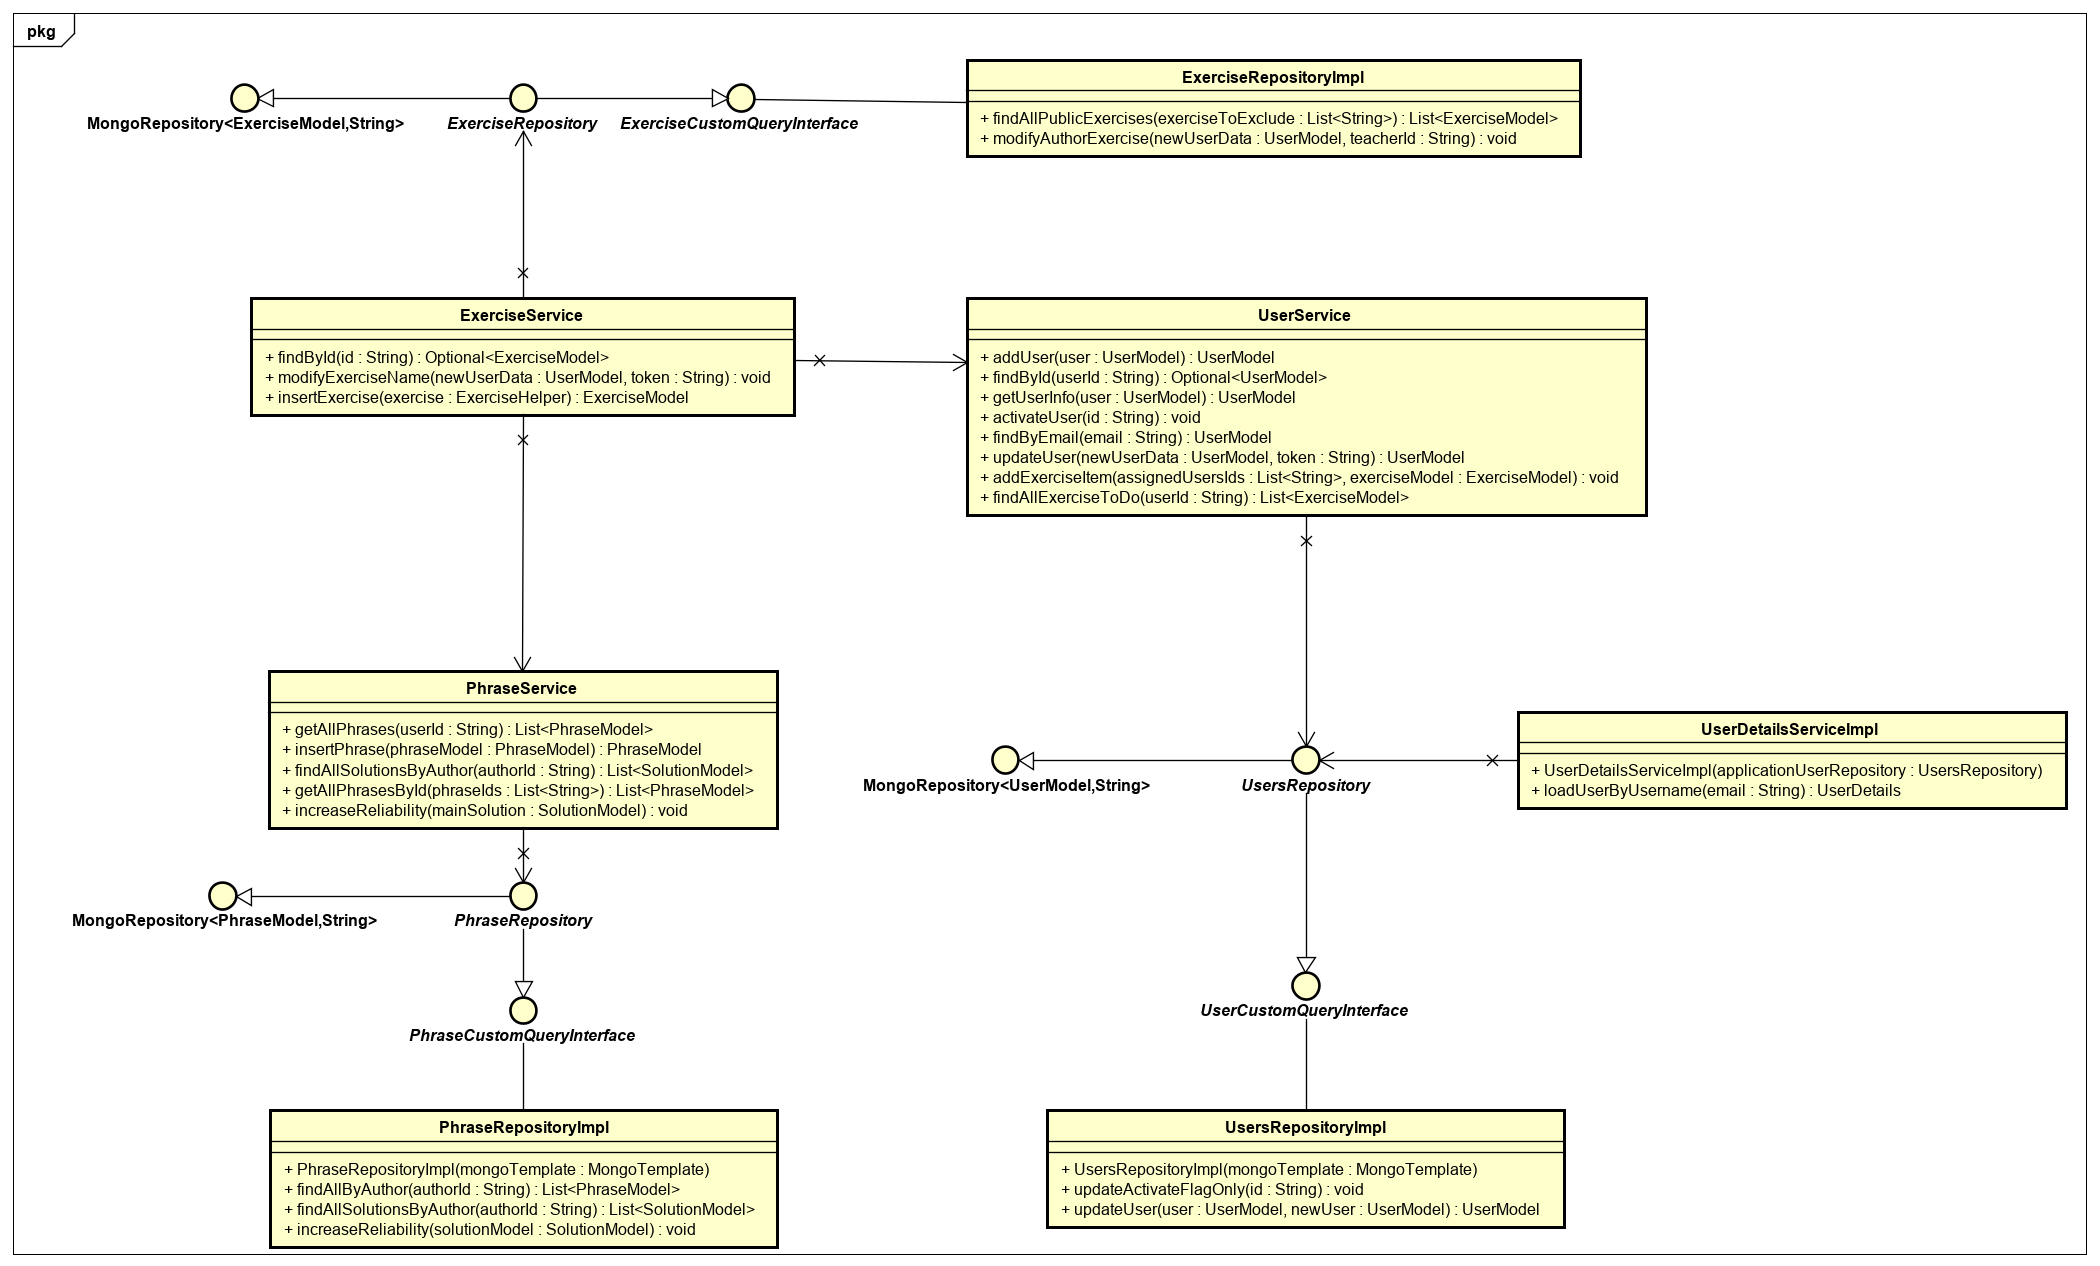
\includegraphics[width=17cm, keepaspectratio]{img/Service-repository.png} 
\caption{Service e Repository}
\end{figure}
\newpage
\subsection{Diagrammi di sequenza}
\subsubsection{Inserimento di un utente}
Il diagramma di sequenza rappresenta l'azione di inserimento di un esercizio nel sistema
\begin{figure}[H]
\centering
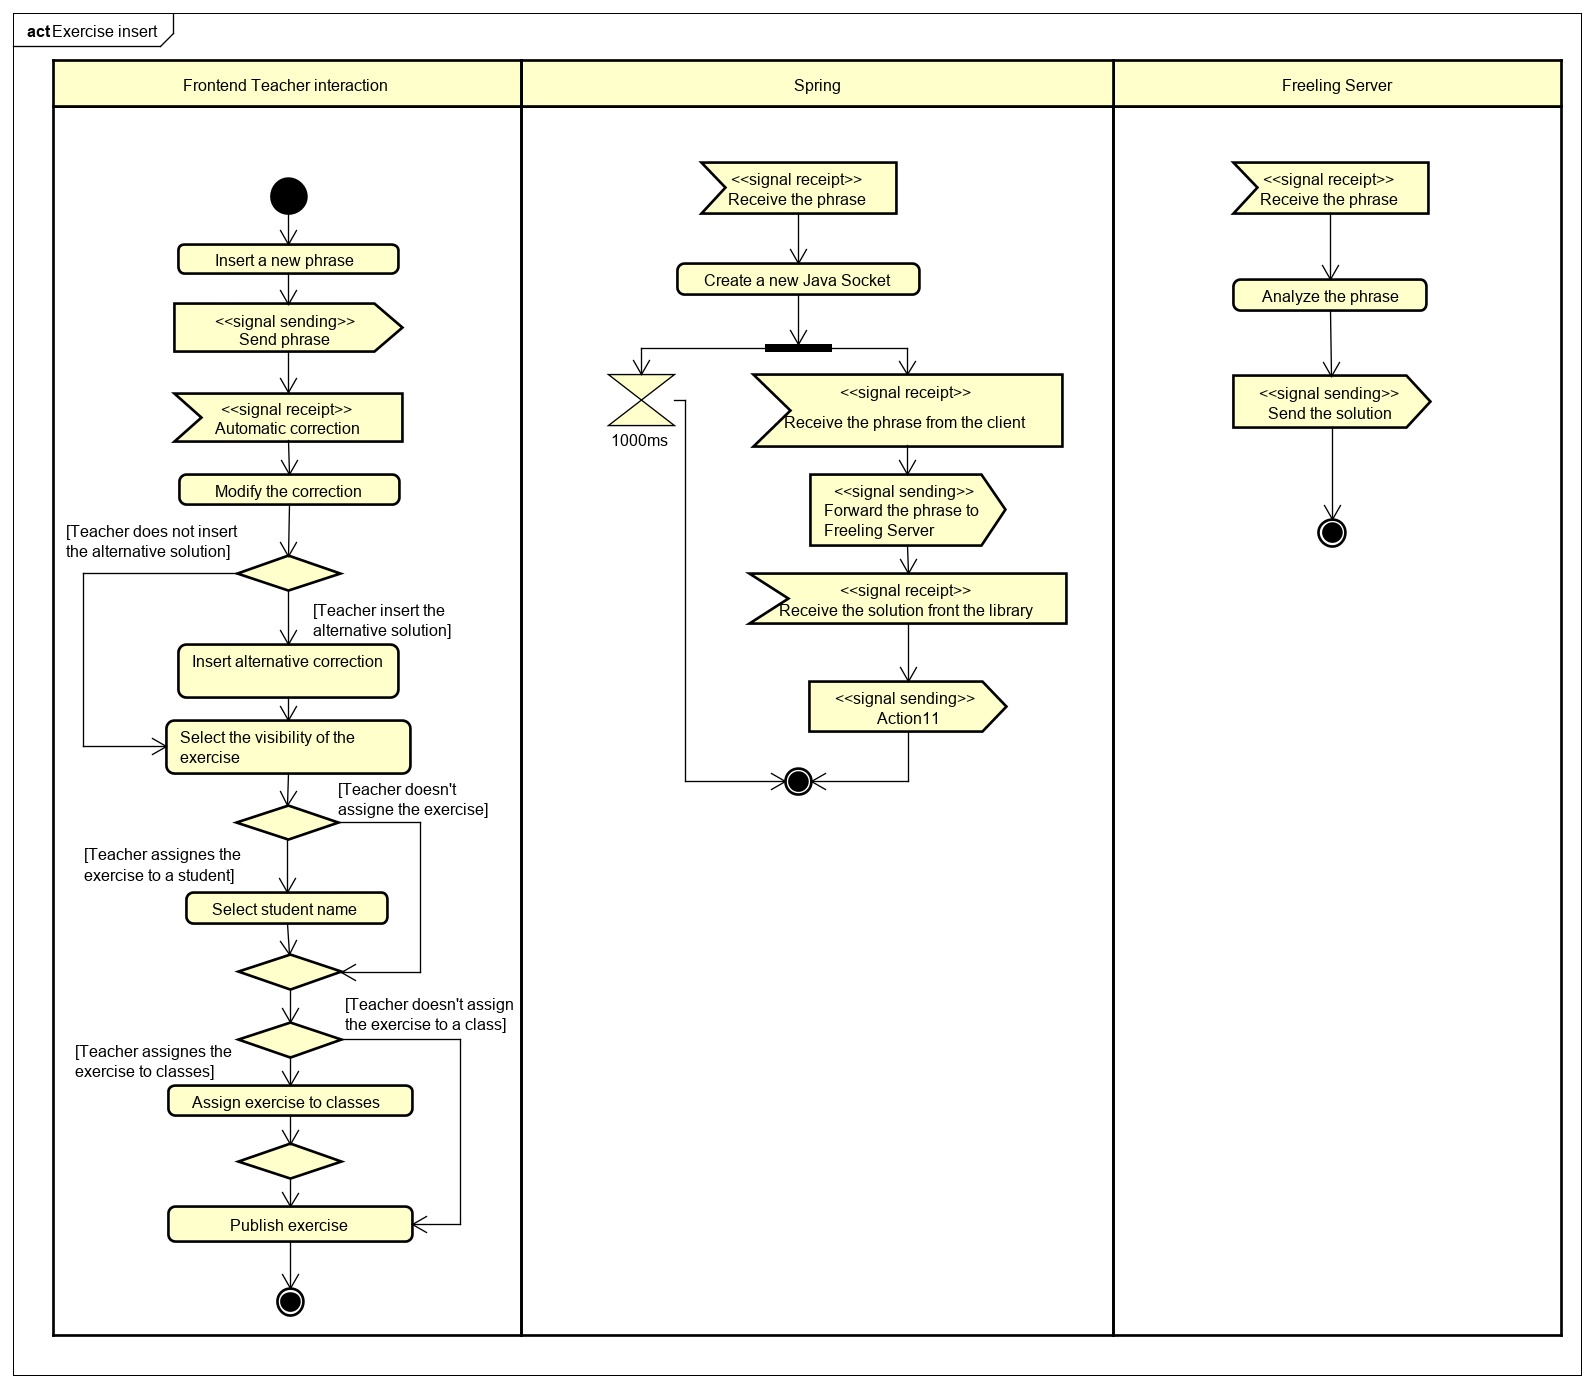
\includegraphics[width=17cm, keepaspectratio]{img/Exercise-insert.png} 
\caption{Exercise insert}
\end{figure}

\begin{figure}[H]
\centering
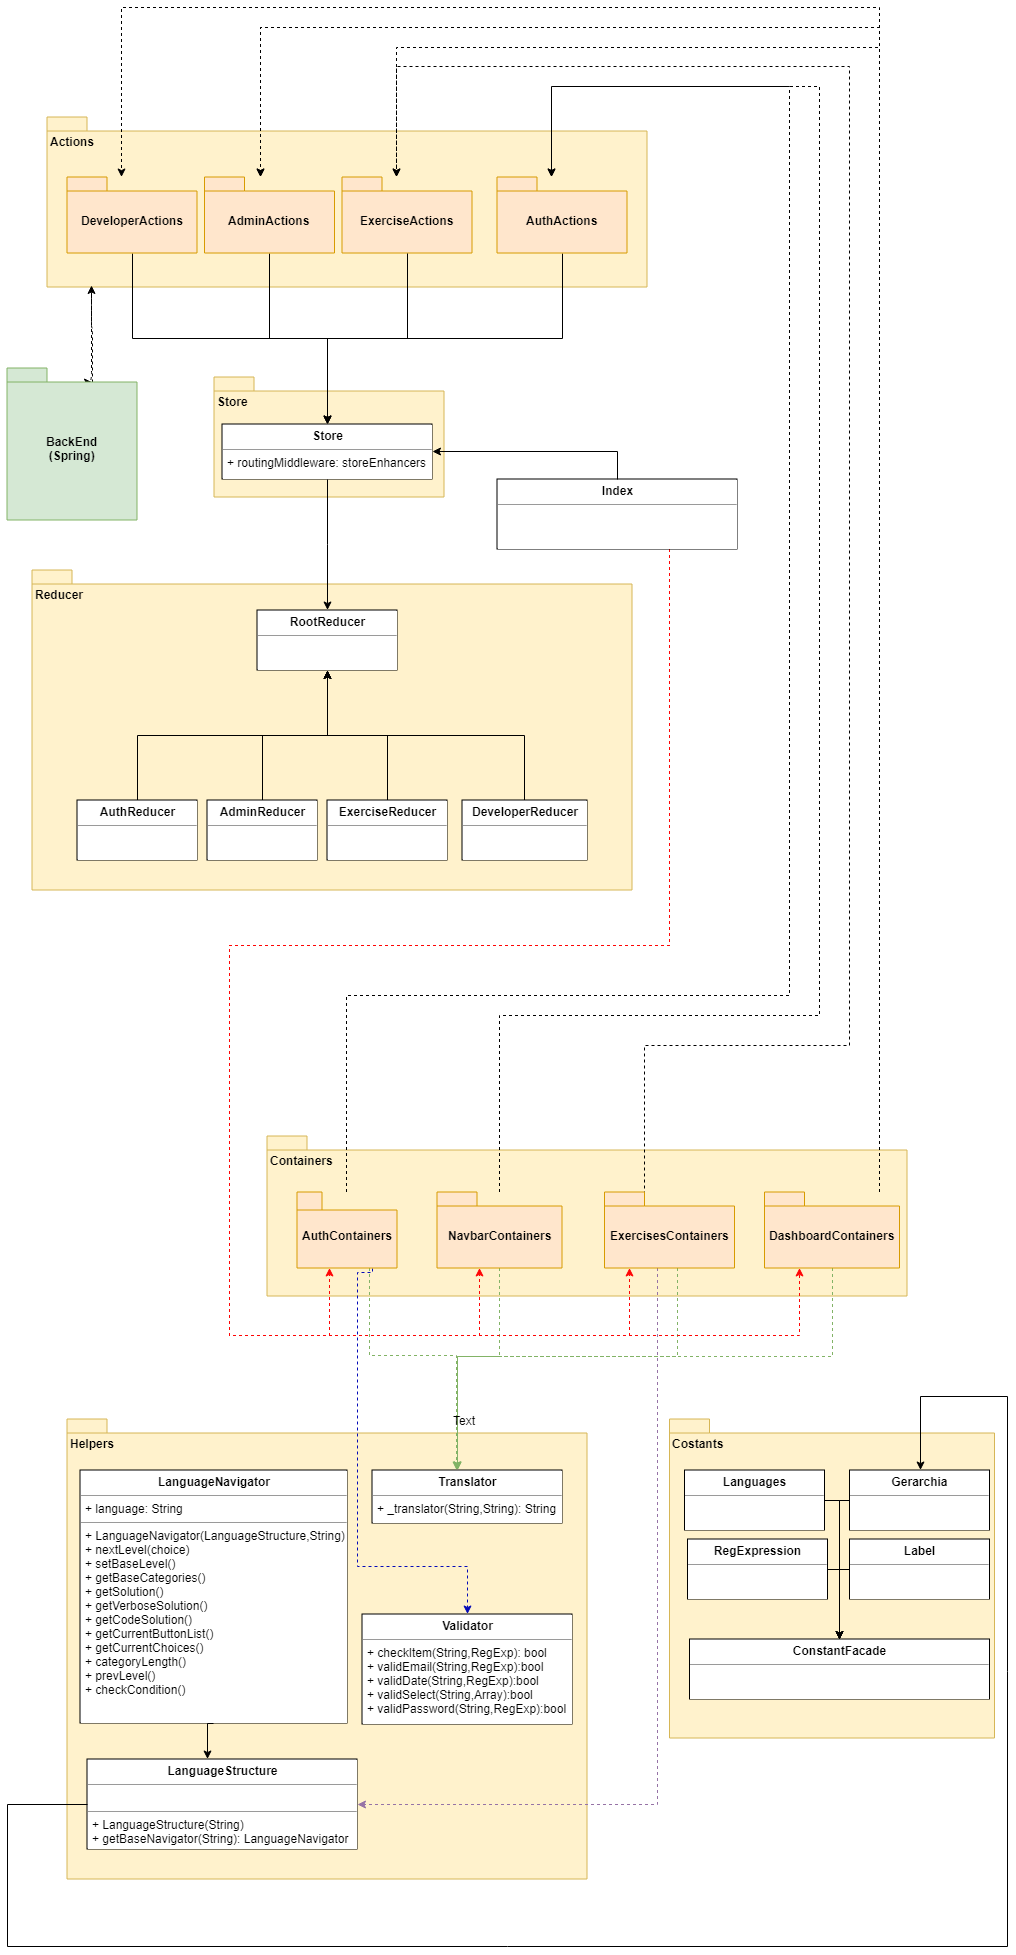
\includegraphics[width=18cm, height=23cm]{img/ReactSpec1.png} 
\caption{UML - FrontEnd}
\end{figure}

\subsubsection{Login}
Il diagramma di sequenza riportato qui di seguito raffigura il processo di login, durante il quale l'utente che vuole accedere può essere autenticato dal sistema.
\begin{figure}[H]
\centering
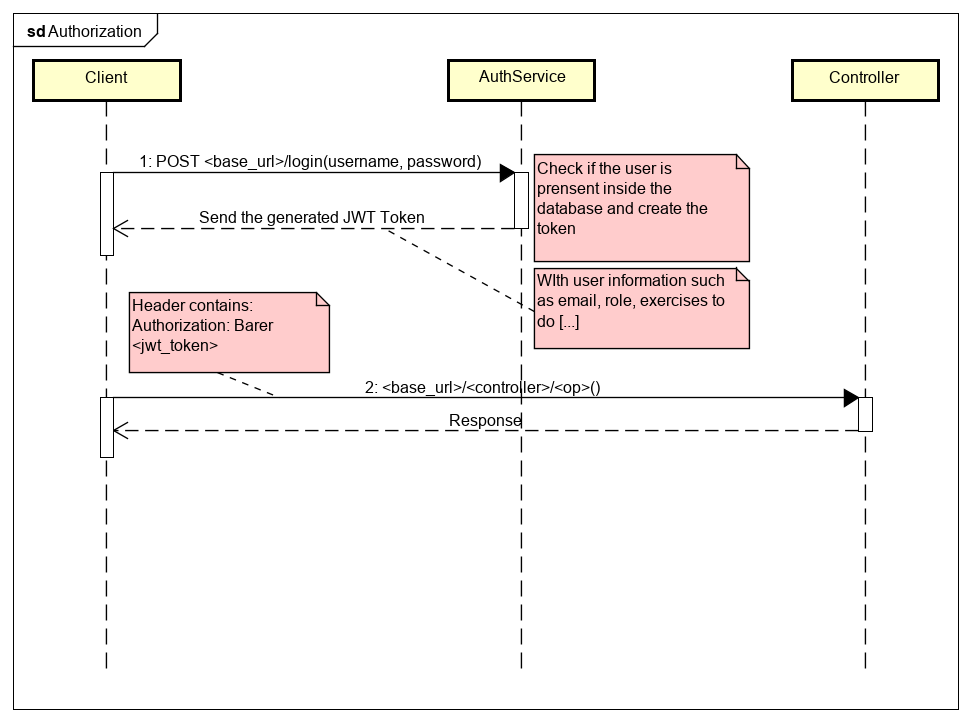
\includegraphics[width=17cm, keepaspectratio]{img/Authorization.png} 
\caption{Authorization}
\end{figure}





\newpage
\section{Diagrammi dei package}
\subsection{Model}
Viene di seguito riportato il diagramma delle classi del package model.
\begin{figure}[H]
\centering
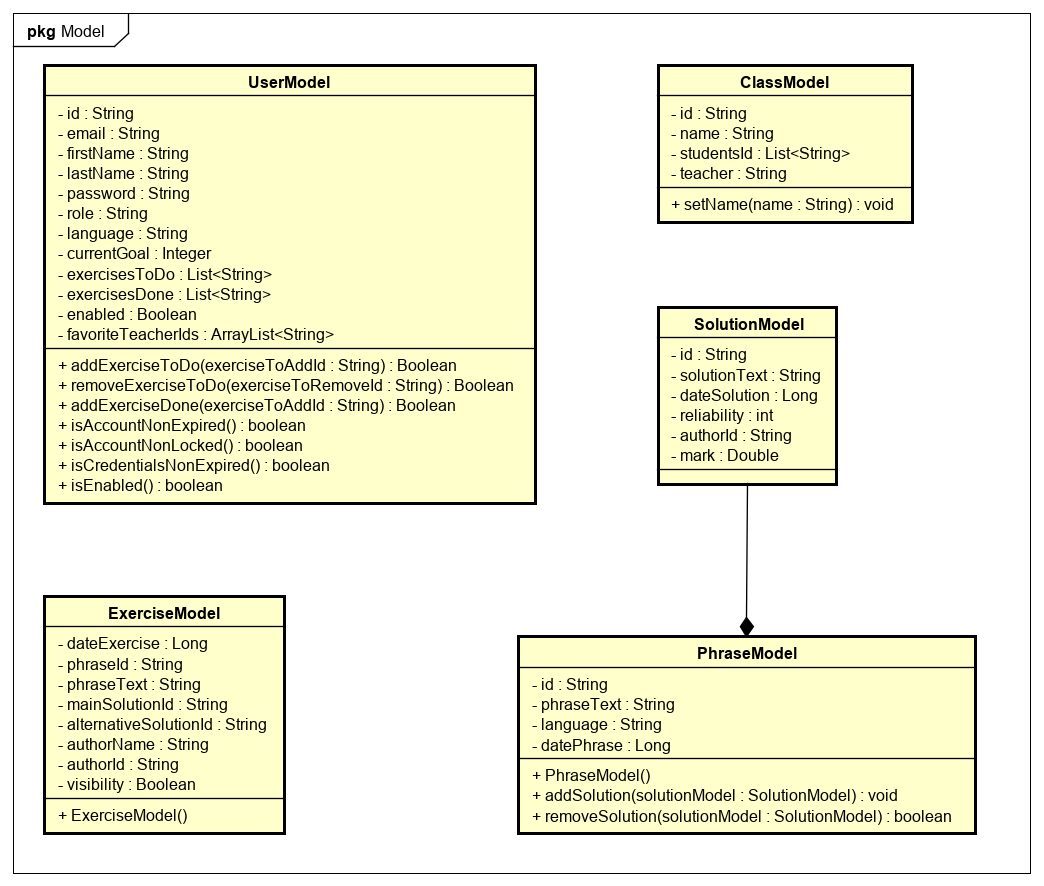
\includegraphics[width=17cm, keepaspectratio]{img/model.png} 
\caption{Model}
\end{figure}
\newpage

\subsection{Controller e service}
Viene di seguito riportato il diagramma delle classi di package controller e service.
\begin{figure}[H]
\centering
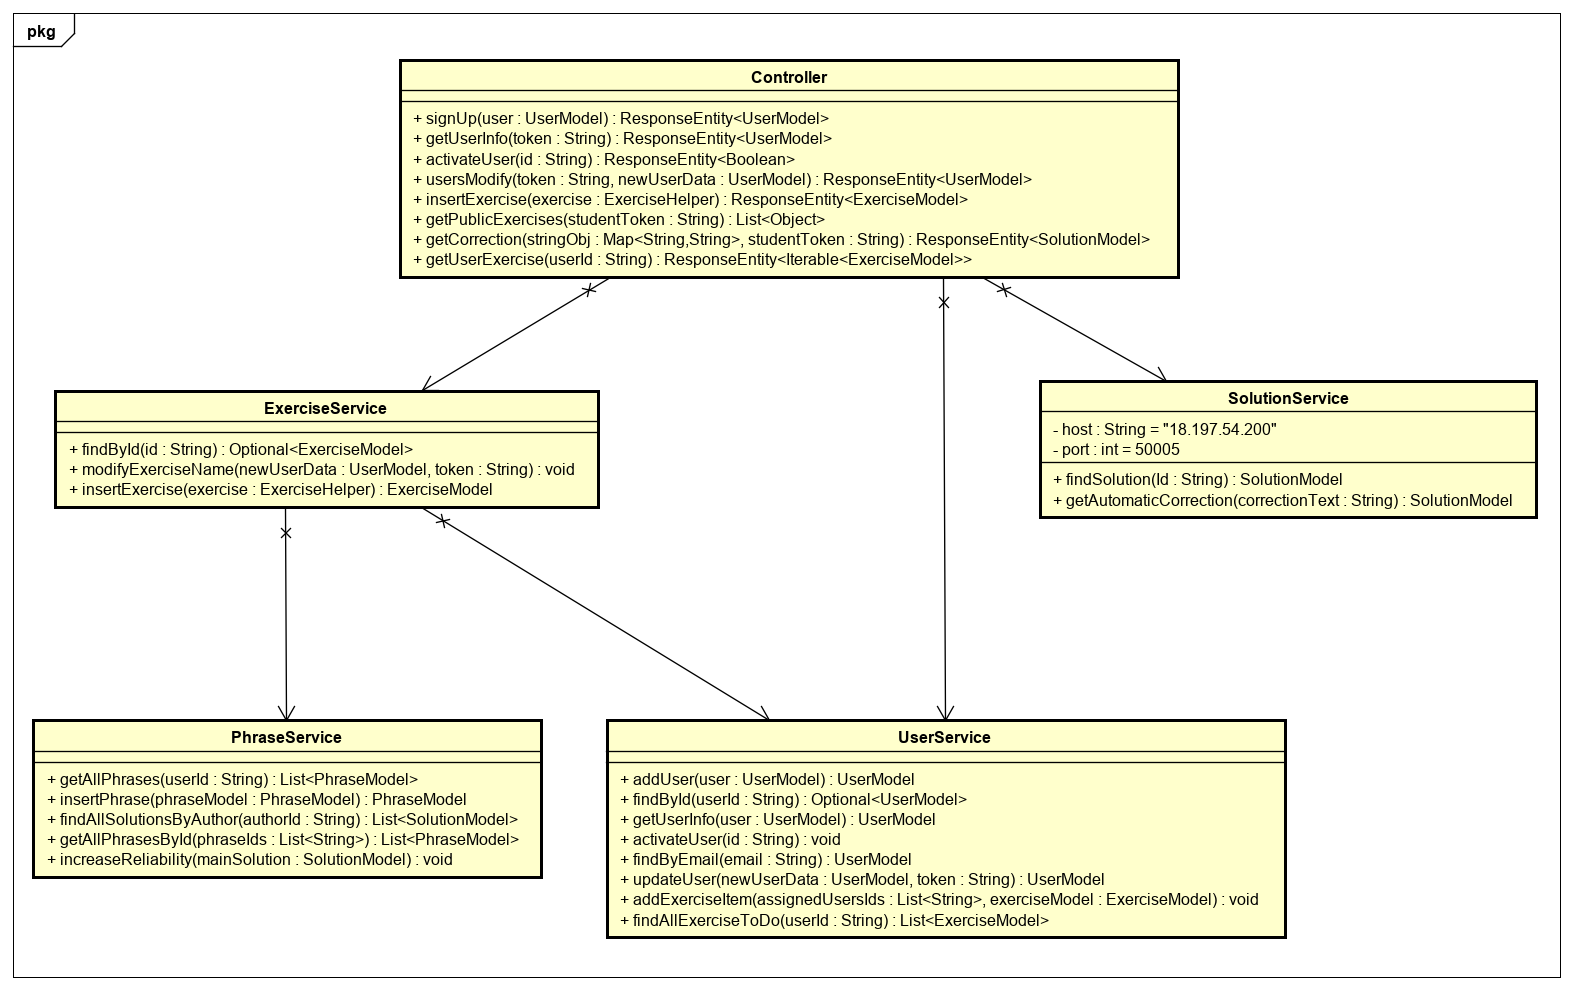
\includegraphics[width=17cm, keepaspectratio]{img/Controller-service.png} 
\caption{Controller e Service}
\end{figure}
\newpage
\subsection{Service e repository}
Viene di seguito riportato il diagramma delle classi di package service e repository.
\begin{figure}[H]
\centering
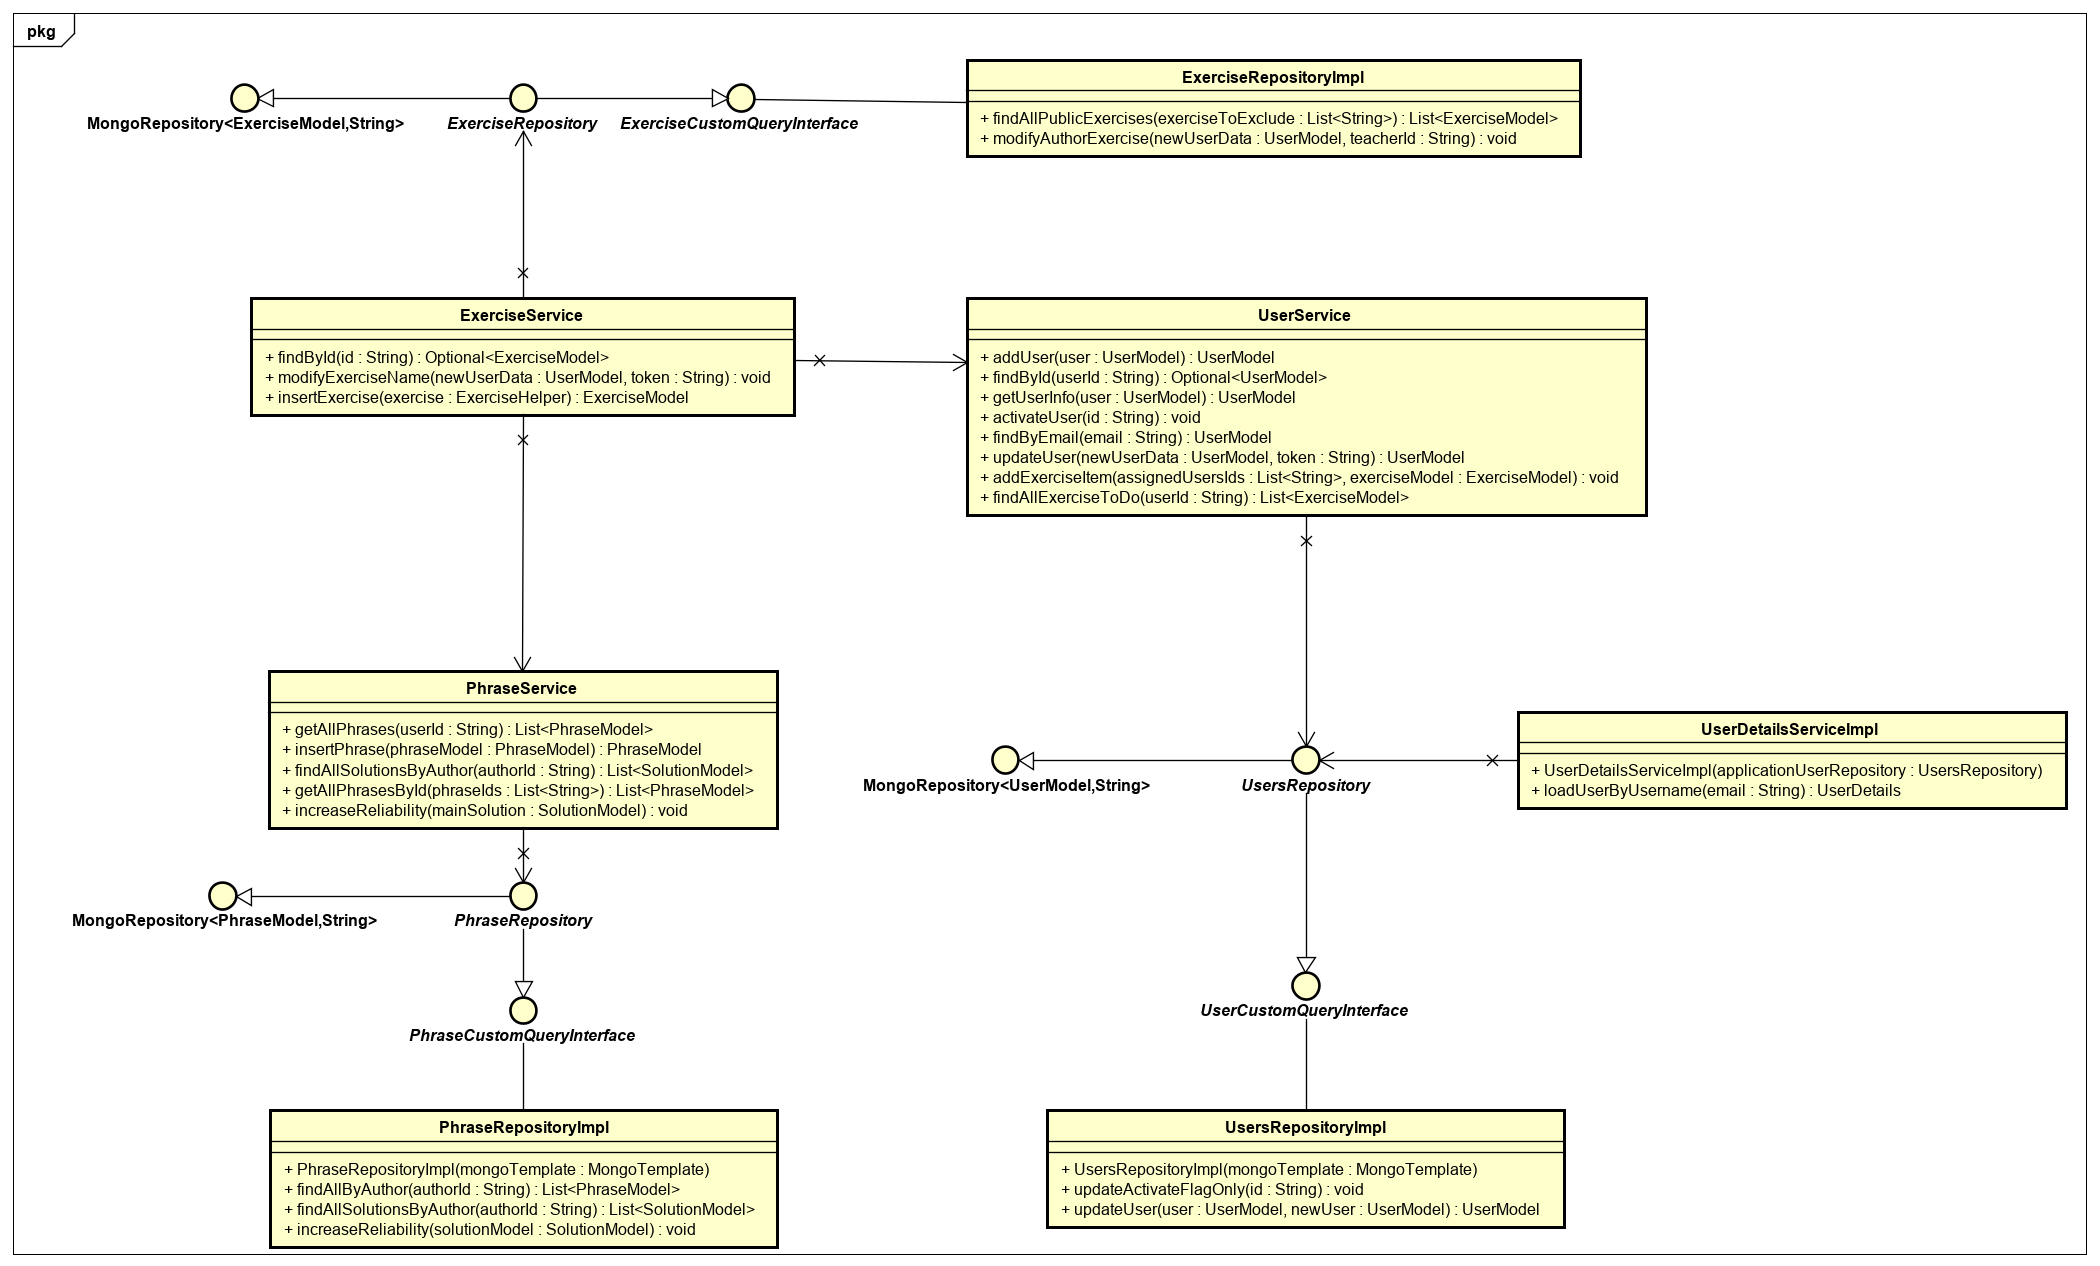
\includegraphics[width=17cm, keepaspectratio]{img/Service-repository.png} 
\caption{Service e Repository}
\end{figure}
\newpage
\section{Diagrammi delle classi e di sequenza}
\subsection{Inserimento di un utente}
Il diagramma di sequenza rappresenta l'azione di inserimento di un esercizio nel sistema
\begin{figure}[H]
\centering
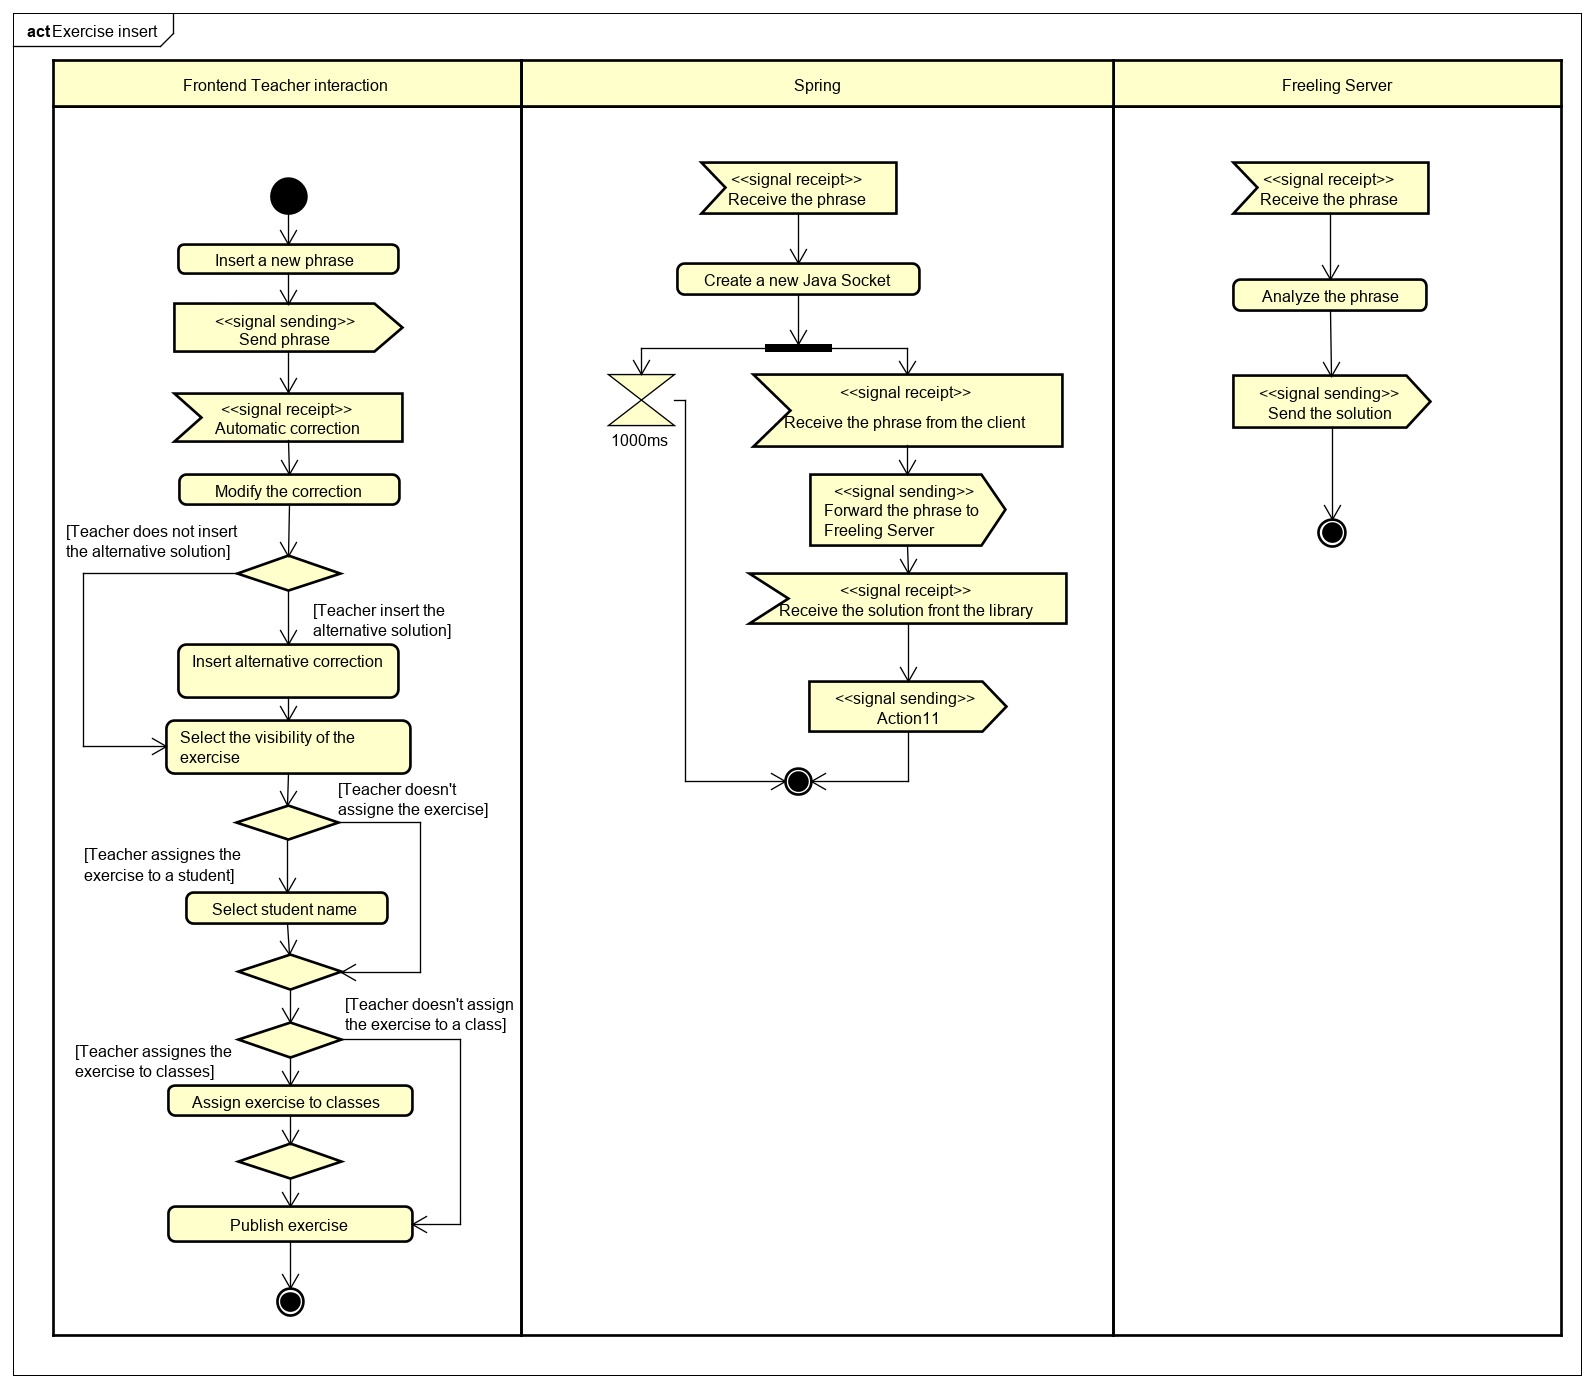
\includegraphics[width=17cm, keepaspectratio]{img/Exercise-insert.png} 
\caption{Exercise insert}
\end{figure}

\begin{figure}[H]
\centering
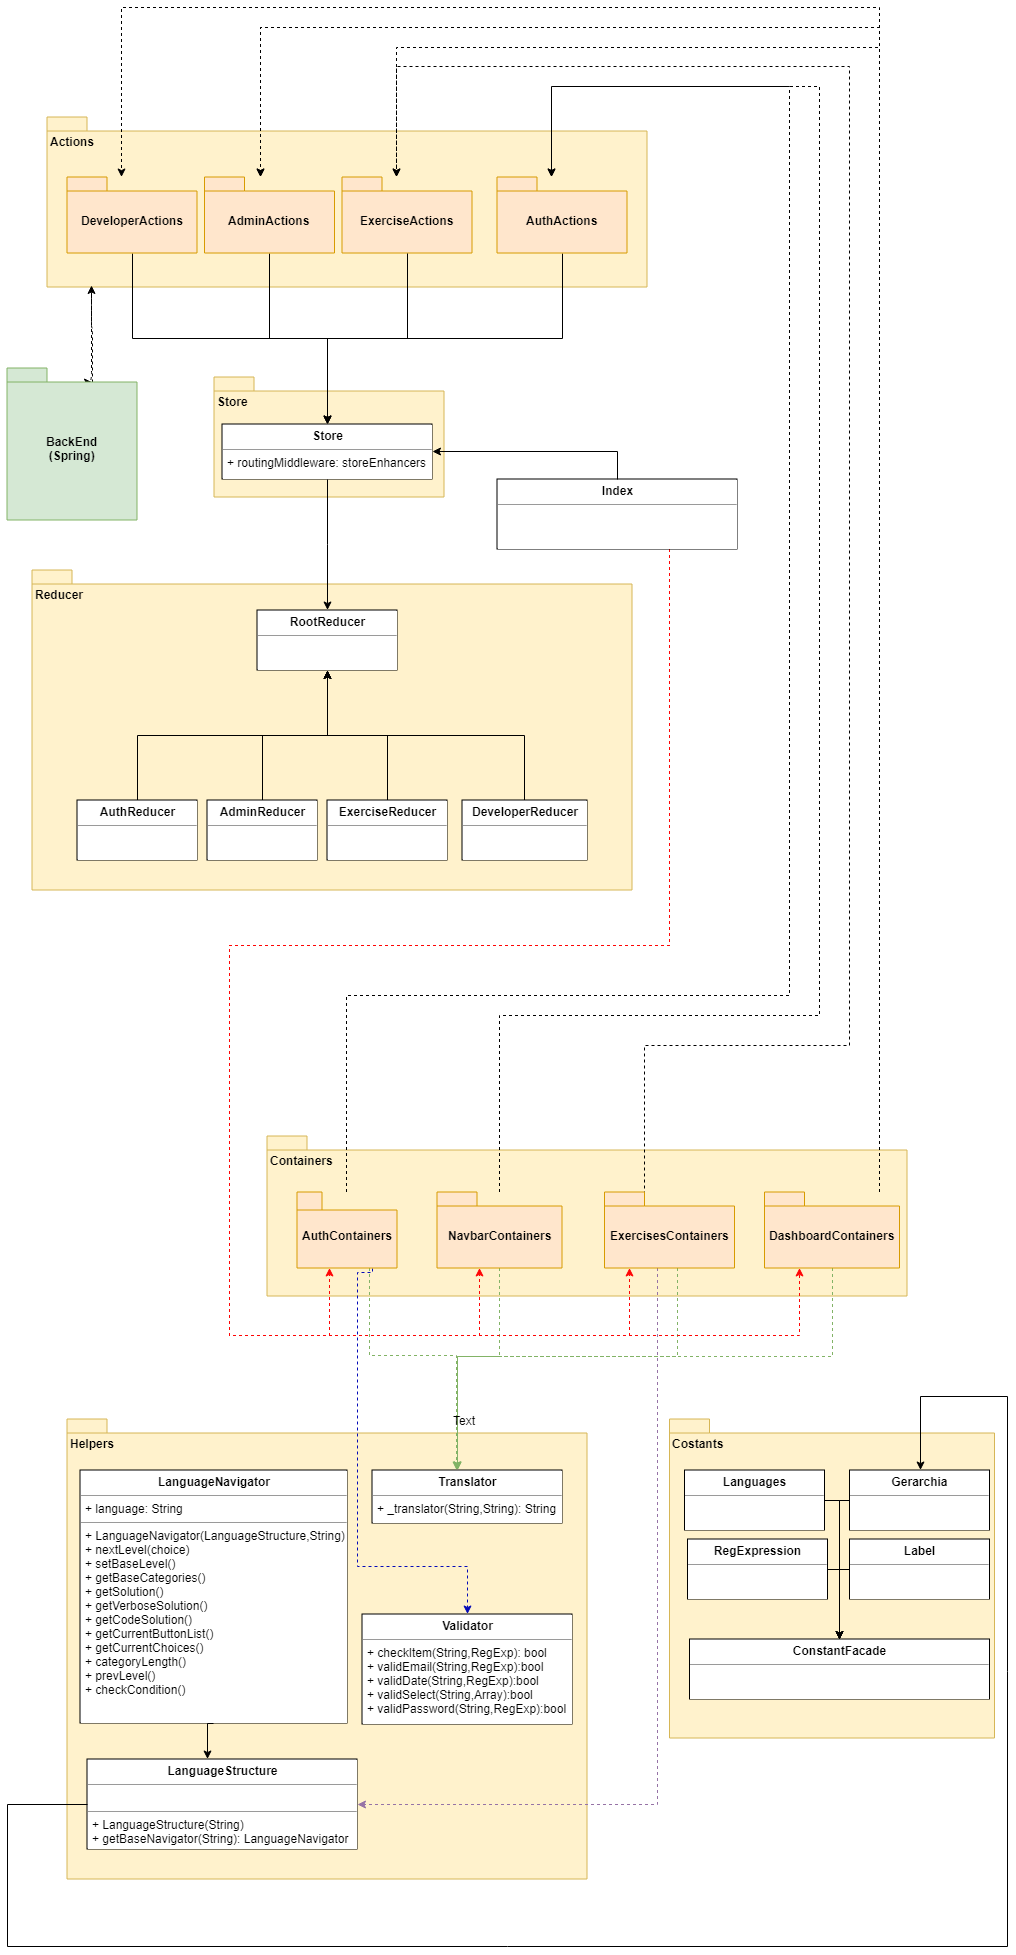
\includegraphics[width=18cm, height=23cm]{img/ReactSpec1.png} 
\caption{UML - FrontEnd}
\end{figure}

\subsection{Login}
Il diagramma di sequenza riportato qui di seguito raffigura il processo di login, durante il quale l'utente che vuole accedere può essere autenticato dal sistema.
\begin{figure}[H]
\centering
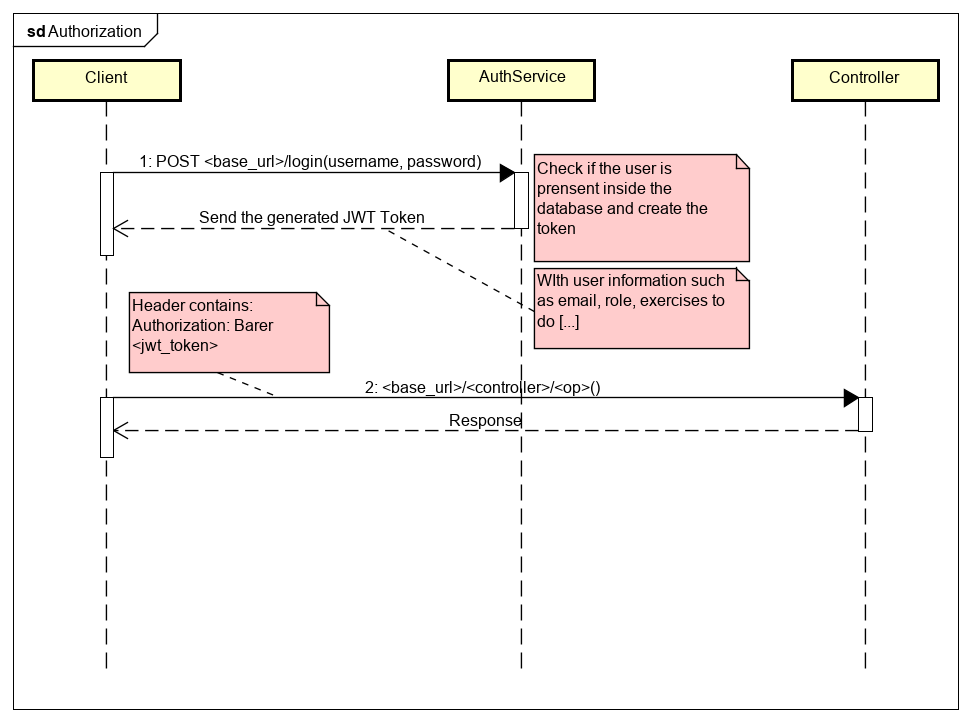
\includegraphics[width=17cm, keepaspectratio]{img/Authorization.png} 
\caption{Authorization}
\end{figure}


\newpage


\end{document}


